% Do NOT change this "Section" title
% and do NOT add more "Section" level titles.
\section{Implementation}\label{sec:implementation}
The implementation has the following parts :

% You can use how many "subsections" and "subsubsections" you like.
\subsection{Hydrophone array}
The hydrophones that have been used in the Naiad AUV are made by Aquarian Audio Products. It has sensor that is capable of picking up sounds from below 20Hz to over 100KHz. Based on the arrival time of the signals of each hydrophone, the sound source can be able to located. When multiple sound sources are present, a beamforming technique can be used to locate the individual sound sources. \newline
With an array of 4 hydrophones, the sound source can be localized. The arrangement chosen is a rectangular array of hydrophones. The length and width of the rectangle is 20mm and 15mm respectively. Since the hydrophone array should detect sound frequencies of upto 30kHz, and considering the speed of sound in water to be 1500 m/s, the minimum distance between the hydrophones can be calculated by:
\begin{center}
$\dfrac{1500}{30000 * 2}$ = 25mm.
\end{center}

The advantages of chosing a rectangular array are:\begin{enumerate}
\item The multilateration algorithm is simplified.
\item It was easy to mount the hydrophones on the AUV.
\end{enumerate}
The disadvantages of the rectangular arrangement is that the accuracy of the algorithm decreases as the source comes closer to the plane of the hydrophones. 


\subsection{Hydrophone Circuit}
The hydrophone circuit includes three smaller circuits, namely:
\begin{itemize}
   \item { \em Bridge amplifier circuit.}
   \item { \em Low pass filter. }
   \item { \em Schmitt trigger circuit. }
\end{itemize}
\subsubsection{Bridge amplifier circuit }
The hydrophone circuit is powered by the +12 and -12 Volt feed from the Power supply board. The amplifier circuit used OP amp named OP42GPZ - OP AMP. This op-amp is a fast precision JFET( The junction gate field-effect transistor )input operational amplifier.\newline
According to typical performance characteristics and electrical characteristics, the gain bandwidth of this product is 10 MHz. This band width is suitable for hydrophone circuit.\newline
In the rectifier circuit care has been taken to attain a high precision signal by using a Schottky diode, that is characterized by a low voltage drop and fast switching time.
The result that has been achieved by using a Schottky diode is more accurate than using other types of diodes.  

\subsubsection{Low pass filter}
Since the low pass filters only allows low frequencies to pass and attenuates frequencies higher than the cutoff frequency,this means that the Hydrophone circuit will pass just a limited range of frequencies to avoid noises or other sounds. Any noise on the hydrophone circuit will decrease accuracy.    
 
 \subsubsection{Schmitt trigger  circuit}
The operational amplifier used in the circuit is the \newline TL084BCNG4 - IC, op-amp. This operational amplifier designed with high slew rates 13V/$\mu s$, supply voltage +12 and -12 Volt and 3 MHz bandwidth that covers the frequency range of the hydrophone circuit.
The Schmitt trigger that will be achieved from circuit will be records the time the signal arrived by the hydrophone software by using external interrupts.
 
%\subsubsection{Subsubsection1}
%Test of one column figure. It should be shown as close as possible to this
%text. If you can't see the figure its number is \ref{fig:one_column_figure}
%and located on page \pageref{fig:one_column_figure}.

%\begin{figure}[h]
%    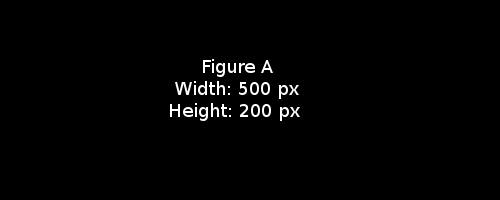
\includegraphics[width=0.5\textwidth]{./figure/figureA.png}
%   \caption{Figure A}
%   \label{fig:one_column_figure}
%\end{figure}

\subsection{Hydrophone software}
The hydrophone software should accept the pulses generated by the hydrophone circuit as input and output the location of the sound source on the CAN bus. The hydrophone software can be divided into 3 modules:
\begin{enumerate}
\item \textbf{External Interrupt:} The hydrophone circuit generates pulses when it gets a sound signal that is above the threshold. The hydrophone circuit is connected to the external interrupt pins of the CAN micro controller. The external interrupt is configured to generate an interrupt on the rising edge. The time of the interrupt occurrence and the number of the hydrophone is pushed in a queue. Whenever the read data is called the data is removed from the queue and returned in FIFO order.
\item \textbf{Multilateration Algorithm:} The multilateration algorithm is initailized by passing the velocity of sound and the length and width of the rectangular array of hydrophones. After initialization the algorithm is executed by calling the \textit{run} function. The \textit{run} function takes the time of arrival of the signals at the hydrophones as input. Care must be taken to ensure that the order of the time of arrival is correct. For example Ti is the time for the hydrophone at (0,0) while Tl is the time for the hydrophone at (l,b). The algorithm returns the sound source location in x,y and z co-orfinates in millimeters. A boolean variable is also returned to tell if the position is correct or not.
\item \textbf{The main program:} The main program initializes the CAN drivers and the external interrupts. It then reads data from the queue of the external interrupts. When it has the data for all the hydrophones it calls the \textit{run} to start the multilateration algorithm. If the valid position is returned it is put out on the CAN bus.
\end{enumerate}

\subsection{Multilateration algorithm simulation}

Since the clocks in any microcontroller has a maximum frequency,a simulation was done in MATLAB to analyse how the clock resolution effects the algorithm. The simulation takes the following inputs the length and width of the rectangular array of hydrophones, the velocity of sound and the location of sound source in 3 dimensions with one of the hydrophones at the origin. Then it calculates the time it will take for the sound from the source to reach the hydrophones. The time is then rounded off to the desired accuracy (currently it is set to micro seconds). By using the rounded off times the location of the sound source is re-calculated. The errors in the original position and calculated position can be observed.\newline
From the simulations it was observed that the AT90CAN128 which has an external clock of 16MHz is too slow to get a fairly accurate estimation of position.\newline It was observed that the minimum clock required to have acceptable errors in localization is 1 GHz. Hence the code was not tested on AT90CAN128.
%\subsubsection{Subsubsection1}
%